\documentclass{assignment}
\ProjectInfos{非线性光学}{PHYS5252P}{2021-2022 学年第二学期}{作业一}{(随堂测验)}{陈稼霖}[https://github.com/Chen-Jialin]{SA21038052}

\begin{document}
\begin{prob}
    利用 KDP 晶体进行参量放大, 若其中有两个光波是 e 光, 第三个光波是 o 光, 试推导相位匹配角公式, 其中信号、空闲和泵浦光中哪一个为寻常光? 令 $\omega_3=$\SI{10000}{cm^{-1}}, $\omega_1=\omega_2=$\SI{5000}{cm^{-1}} 能否实现这种形式的相位匹配?
\end{prob}
\begin{sol}
    KDP 为负单轴的晶体, 故为 II 类相位匹配 ($e+o\rightarrow e$).

    要实现相位匹配, 需满足
    \begin{align}
        \frac{1}{2}[n_e^{\omega}(\theta)+n_o^{\omega}]=n_e^{2\omega}(\theta_m),
    \end{align}
    其中传播方向与光轴夹角为 $\theta$ 的非常光的折射率满足
    \begin{align}
        \frac{1}{[n_e^{\omega\text{ 或 }2\omega}(\theta)]^2}=\frac{\cos^2\theta}{n_o^2}+\frac{\sin^2\theta}{[n_e^{\omega\text{ 或 }2\omega}(\theta)]^2}.
    \end{align}
    由于 $n_o^{\omega}=1.4596$, $n_e^{\omega}=1.4606$, $n_e^{2\omega}=1.4999$, $\frac{1}{2}[n_e^{\omega}(\pi/2)+n_o^{\omega}]<n_e^{2\omega}(\pi/2)$, 故无角度满足相位匹配条件, 无法实现相位匹配.
\end{sol}

\begin{prob}
    试证明外加直流电场 $E_x=E_{0j}$ 的 KDP 晶体, 光波在 $zox$ 面内、与 $x$ 轴成 $45^{\circ}$ 方向传播时的电光延迟为下式. 其中 $l$ 为沿光传播方向上的晶体长度, $d$ 为沿外加电场的晶体厚度, $U_y$ 为外加电压.
    \[
        \Delta\varphi\approx\frac{2\pi l}{\lambda}\left[\frac{\sqrt{2}n_on_e}{\sqrt{n_o^2+n_e^2}}-n_o+\sqrt{2}\left[\frac{1}{n_o^2}+\frac{1}{n_e^2}\right]^{-3/2}\gamma_{41}U_y\frac{l}{d}\right].
    \]
\end{prob}
\begin{pf}
    KDP 为负单轴晶体, 故无外加电场下, KDP 折射率椭球方程为
    \begin{align}
        \frac{x^2}{n_o^2}+\frac{y^2}{n_o^2}+\frac{z^2}{n_e^2}=1,
    \end{align}
    光波在 $zox$ 面内、与 $x$ 轴成 $45^{\circ}$ 方向传播时, 垂直于 $zox$ 面的偏振分量感受到的折射率为 $n_{\perp}=n_o$, 平行于 $zox$ 面的折射率分量感受到的折射率满足
    \begin{gather}
        \frac{n_{\parallel}^2\sin^2(-45^{\circ})}{n_o^2}+\frac{n_{\parallel}^2\cos^2(-45^{\circ})}{n_e^2}=1,\\
        \Longrightarrow n_{\parallel}=\frac{\sqrt{2}n_on_e}{\sqrt{n_o^2+n_e^2}}.
    \end{gather}
    KDP 的电光系数为
    \begin{align}
        [\gamma_{ij}]=\begin{bmatrix}
            0&0&0\\
            0&0&0\\
            0&0&0\\
            \gamma_{41}&0&0\\
            0&\gamma_{41}&0\\
            0&0&\gamma_{63}
        \end{bmatrix},
    \end{align}
    故外加电场 $E_x=E_{0j}=\frac{U_y}{d}$ 下, KDP 折射率椭球系数变化量为
    \begin{align}
        \begin{bmatrix}
            \Delta\left(\frac{1}{n^2}\right)_1\\
            \Delta\left(\frac{1}{n_2}\right)_2\\
            \Delta\left(\frac{1}{n_2}\right)_3\\
            \Delta\left(\frac{1}{n_2}\right)_4\\
            \Delta\left(\frac{1}{n_2}\right)_5\\
            \Delta\left(\frac{1}{n_2}\right)_6
        \end{bmatrix}=\begin{bmatrix}
            0&0&0\\
            0&0&0\\
            0&0&0\\
            r_{41}&0&0\\
            0&r_{41}&0\\
            0&0&r_{63}
        \end{bmatrix}\begin{bmatrix}
            E_{0j}\\
            0\\
            0
        \end{bmatrix}=\begin{bmatrix}
            0\\
            0\\
            0\\
            0\\
            \gamma_{41}E_{0j}\\
            0
        \end{bmatrix},
    \end{align}
    折射率椭球方程为
    \begin{align}
        \frac{x^2}{n_o^2}+\frac{y^2}{n_o^2}+\frac{z^2}{n_e^2}+2\gamma_{41}E_{0j}xz=1,
    \end{align}
    光波在 $zox$ 面内、与 $x$ 轴成 $45^{\circ}$ 方向传播时, 垂直于 $zox$ 面的偏振分量感受到的折射率满足
    \begin{align}
        \frac{[n_{\perp}']^2}{n_o^2}=1,\\
        \Longrightarrow n_{\perp}'=n_o,
    \end{align}
    平行于 $zox$ 面的偏振分量感受到的折射率满足
    \begin{gather}
        \frac{[n_{\parallel}']^2\sin^2(-45^{\circ})}{n_o^2}+\frac{[n_{\parallel}']^2\cos^2(-45^{\circ})}{n_e^2}+2\gamma_{41}E_{0j}n_{\parallel}'\sin(-45^{\circ})n_{\parallel}'\cos(-45^{\circ})=1,\\
        \Longrightarrow n_{\parallel}'=\frac{1}{\sqrt{\frac{n_o^2+n_e^2}{2n_o^2n_e^2}-r_{41}E_{0j}}}=\frac{\sqrt{2}n_on_e}{\sqrt{n_e^2+n_o^2}}\frac{1}{\sqrt{1-\frac{2n_o^2n_e^2}{n_e^2+n_o^2}r_{41}E_{0j}}}\approx\sqrt{2}\frac{n_on_e}{\sqrt{n_o^2+n_e^2}}+\sqrt{2}\left(\frac{n_o^2n_e^2}{n_o^2+n_e^2}\right)^{3/2}\gamma_{41}E_{0j},
    \end{gather}
    故电光延迟为
    \begin{align}
        \Delta\varphi=\frac{2\pi l(n_{\parallel}'-n_{\perp}')}{\lambda}\approx\frac{2\pi l}{\lambda}\left[\frac{\sqrt{2}n_on_e}{n_o^2+n_e^2}-n_o+\sqrt{2}\left[\frac{1}{n_o^2}+\frac{1}{n_e^2}\right]^{-3/2}\gamma_{41}\frac{U_y}{d}\right].
    \end{align}
\end{pf}

\begin{prob}
    考虑 \ce{LiNbO_3} 浸提中的 II 型 ($o+e\rightarrow e$) 相位匹配下的共线传播倍频过程 $\omega+\omega\rightarrow 2\omega$:
    \begin{itemize}
        \item[1)] 设光波矢沿 $(\theta,\varphi)$, 求出此时有效非线性系数 $d_{\text{eff}}$ 的表达式.
        注: 已知 \ce{LiNbO_3} 晶体 (负单轴晶体) 的非线性系数矩阵为
        \[
            \begin{Bmatrix}
                0&0&0&0&d_{15}&-d_{22}\\
                -d_{22}&d_{22}&0&d_{15}&0&0\\
                d_{31}&d_{31}&d_{33}&0&0&0
            \end{Bmatrix}.
        \]
        \item[2)] 用折射率曲面的方法画出实现相位匹配的示意图.
        \item[3)] 若要得到最佳倍频输出, 问光波矢的方向 $(\theta,\varphi)$ 应取何值?
    \end{itemize}
\end{prob}
\begin{sol}
    \begin{itemize}
        \item[1)] 
        \begin{align}
            \bm{a}^o=&\begin{bmatrix}
                \sin\varphi\\
                -\cos\varphi\\
                0
            \end{bmatrix},\\
            \bm{a}^e=&\begin{bmatrix}
                -\cos\theta\cos\varphi\\
                -\cos\theta\sin\varphi\\
                \sin\theta
            \end{bmatrix},\\
            \bm{a}^o\bm{a}^e=&\begin{bmatrix}
                -\cos\theta\sin\varphi\cos\varphi\\
                -\cos\theta\sin\varphi\cos\varphi\\
                0\\
                -2\sin\theta\cos\varphi\\
                2\sin\theta\sin\varphi\\
                \cos\theta\cos 2\varphi
            \end{bmatrix}.
        \end{align}
        II 型相位匹配下, 有效非线性系数为
        \begin{align}
            \notag d_{eff}=&\bm{a}^e\cdot\begin{bmatrix}
                0&0&0&0&d_{15}&-d_{22}\\
                -d_{22}&d_{22}&0&d_{15}&0&0\\
                d_{31}&d_{31}&d_{33}&0&0&0
            \end{bmatrix}\bm{a}^o\bm{a}^e\\
            \notag=&\begin{bmatrix}
                -\cos\theta\cos\varphi&-\cos\theta\sin\varphi&\sin\theta
            \end{bmatrix}\begin{bmatrix}
                0&0&0&0&d_{15}&-d_{22}\\
                -d_{22}&d_{22}&0&d_{15}&0&0\\
                d_{31}&d_{31}&d_{33}&0&0&0
            \end{bmatrix}\begin{bmatrix}
                -\cos\theta\sin\varphi\cos\varphi\\
                -\cos\theta\sin\varphi\cos\varphi\\
                0\\
                -2\sin\theta\cos\varphi\\
                2\sin\theta\sin\varphi\\
                \cos\theta\cos 2\varphi
            \end{bmatrix}\\
            \notag=&\begin{bmatrix}
                -\cos\theta\cos\varphi&-\cos\theta\sin\varphi&\sin\theta
            \end{bmatrix}\begin{bmatrix}
                2d_{15}\sin\theta\sin\varphi-d_{22}\cos\theta\cos 2\varphi\\
                -2d_{15}\sin\theta\cos\varphi\\
                -2d_{13}\cos\theta\sin\varphi\cos\varphi
            \end{bmatrix}\\
            =&d_{22}\cos^2\theta\cos\varphi\cos 2\varphi-2d_{13}\cos\theta\sin\theta\sin\varphi\cos\varphi.
        \end{align}
        \item[2)] 如图 \ref{A1-3}.
        \begin{figure}[H]
            \centering
            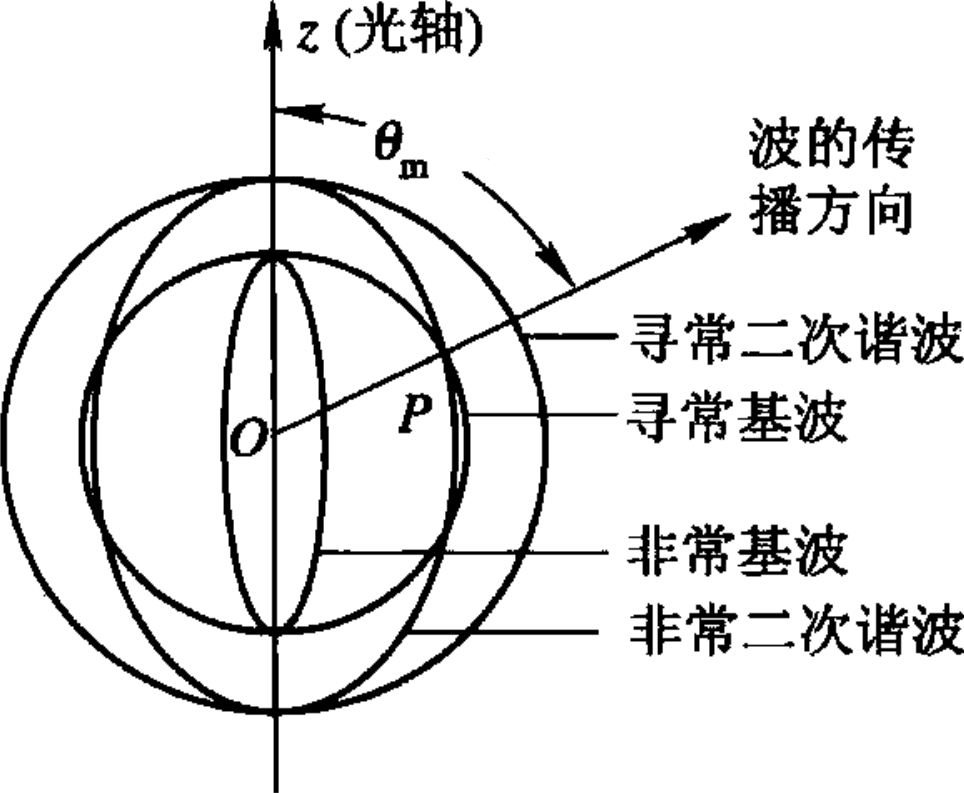
\includegraphics[width=.5\columnwidth]{Figures/A1-3.png}
            \caption{II 型相位匹配示意图.}
            \label{A1-3}
        \end{figure}
        \item[3)] 为得到最佳倍频输出, 取 $\theta_m$ 满足 $\frac{1}{2}[n_e^{\omega}(\theta)+n_o^{\omega}]=n_e^{2\omega}(\theta)$, 在此基础上取 $\varphi$ 使 $d_{eff}$ 极大.
    \end{itemize}
\end{sol}

\begin{prob}
    试证明在非共线相位匹配的条件下, 为获得远红外差频光 ($\omega_1$、$\omega_2\gg\omega_3$), 晶体必须具有反常色散特性.
\end{prob}
\begin{pf}
    为获得远红外差频光, $\omega_1-\omega_2=\omega_3$, $n_1\approx n_2\equiv n$, $n_3\approx n+\Delta n$. 由余弦定理, $\bm{k}_1$ 和 $\bm{k}_2$ 之间的夹角 $\theta$ 满足
    \begin{align}
        \cos\theta=\frac{k_1^2+k^2-k_3^2}{2k_1k_2}=\frac{(n_1\omega_1)^2+(n_2\omega_2)^2-(n_3\omega_3)^2}{2n_1\omega_1n_2\omega_2}\approx\frac{n^2(\omega_1^2+\omega_2^2)-(n+\Delta n)^2(\omega_1-\omega_2)^2}{2n^2\omega_1\omega_2}\approx 1-\frac{\Delta n}{n}\frac{(\omega_1-\omega_2)^2}{\omega_1\omega_2}.
    \end{align}
    由 $\cos\theta<1$ 得 $\Delta n>0$, 即反常色散.
\end{pf}

\begin{prob}
    试证明, 如果二次谐波产生过程的基频光 $\omega$ 是寻常光, 倍频光 $2\omega$ 是非常光, $\theta_m$ 是其相位匹配角, 则有
    \[
        \Delta k(\theta)L|_{\theta=\theta_m}=\frac{2\omega L}{c}\sin(2\theta_m)\frac{(n_e^{2\omega})^{-2}-(n_o^{2\omega})^{-2}}{2(2n_o^{2\omega})^{-3}}(\theta-\theta_m).
    \]
\end{prob}
\begin{pf}
    该过程为负单轴晶体的 I 类相位匹配, 匹配条件为
    \begin{align}
        n_o^{\omega}=n_e^{2\omega}(\theta_m).
    \end{align}
    相位失配为
    \begin{align}
        \Delta k=2\frac{n_o^{\omega}\omega}{c}-\frac{n_e^{2\omega}(\theta)2\omega}{c}=-\frac{2\omega}{c}\frac{\partial n_e^{2\omega}(\theta)}{\partial\theta}(\theta-\theta_m),
    \end{align}
    其中
    \begin{gather}
        \frac{[n_e^{2\omega}(\theta)]^2\cos^2\theta}{[n_o^{2\omega}]^2}+\frac{[n_e^{2\omega}(\theta)]^2\sin^2\theta}{[n_e^{2\omega}]^2}=1,\\
        \Longrightarrow n_e^{2\omega}(\theta)=\frac{n_o^{2\omega}n_e^{2\omega}}{\sqrt{[n_e^{2\omega}]^2\cos^2\theta+[n_o^{2\omega}]^2\sin^2\theta}},
    \end{gather}
    \begin{align}
        \notag\Longrightarrow\frac{\partial n_e^{2\omega}}{\partial\theta}=&-\frac{1}{2}n_o^{2\omega}n_e^{2\omega}\{[n_e^{2\omega}\cos\theta]^2+[n_o^{2\omega}\sin\theta]^2\}^{-3/2}\{[n_o^{2\omega}]^2-[n_e^{2\omega}]^2\}\sin 2\theta\\
        \notag=&-\frac{1}{2}[n_o^{2\omega}]^{-2}[n_e^{2\omega}]^{-2}\left\{\frac{\cos^2\theta}{[n_o^{2\omega}]^2}+\frac{\sin^2\theta}{[n_e^{2\omega}]^2}\right\}^{-3/2}\{[n_o^{2\omega}]^2-[n_e^{2\omega}]^2\}\sin 2\theta\\
        \notag=&-\frac{1}{2}[n_o^{2\omega}]^{-2}[n_e^{2\omega}]^{-2}[n_e^{2\omega}(\theta)]^{-3/2}\{[n_o^{2\omega}]^2-[n_e^{2\omega}]^2\}\sin 2\theta,
    \end{align}
    由于 $n_o^{\omega}=n_e^{2\omega}(\theta_m)$, 故
    \begin{align}
        \notag\frac{\partial n_e^{2\omega}(\theta_m)}{\partial\theta}=&-\frac{1}{2}[n_o^{2\omega}]^{-2}[n_e^{2\omega}]^{-2}[n_e^{2\omega}(\theta_m)]^{-3/2}\{[n_o^{2\omega}]^2-[n_e^{2\omega}]^2\}\sin 2\theta_m\\
        \notag=&-\frac{1}{2}[n_o^{2\omega}]^{-2}[n_e^{2\omega}]^{-2}[n_o^{\omega}]^{-3}\{[n_o^{2\omega}]^2-[n_e^{2\omega}]^2\}\sin 2\theta_m\\
        \notag=&-\frac{1}{2}\frac{[n_e^{2\omega}]^2-[n_o^{2\omega}]^2}{[n_o^{\omega}]^3}\sin 2\theta_m.
    \end{align}
    将上式代回相位适配表达式中得
    \begin{align}
        \Delta k=\frac{2\omega}{c}\frac{[n_e^{2\omega}]^{-2}-[n_o^{2\omega}]^{-2}}{2[n_o^{\omega}]^3}\sin(2\theta_m)(\theta-\theta_m),
    \end{align}
    故
    \begin{align}
        \Delta k(\theta)L|_{\theta=\theta_m}=\frac{2\omega L}{c}\sin(2\theta_m)\frac{(n_e^{2\omega})^{-2}-(n_o^{2\omega})^{-2}}{2(2n_o^{2\omega})^{-3}}(\theta-\theta_m).
    \end{align}
\end{pf}

\begin{prob}
    参量振荡器可以看作是一种新型的激光器, 利用它可以实现频率的调谐输出, 请以负单轴 II 类晶体为例, 分析角度调谐输出.
\end{prob}
\begin{sol}
    
\end{sol}

\begin{prob}
    请以负单轴晶体为例, 按以下条件分别推导 I 型和 II 型二次谐波的匹配带宽:
    \begin{itemize}
        \item[1)] 简并共线;
        \item[2)] 简并非贡献,
    \end{itemize}
    并比较 I 型和 II 型的带宽特点.
\end{prob}
\begin{pf}
    \begin{itemize}
        \item[1)] 
        \item[2)] 
    \end{itemize}
\end{pf}
\end{document}